\subsection{YugaByteDB}

YugaByteDB merupakan basis data relasional terdistribusi dengan konsensus Raft. YugaByteDB memenuhi prinsip ACID dan terdistribusi secara \textit{native}. YugaByteDB kompatibel dengan API Cassandra (YCQL) dan API Postgres (YSQL).

YugaByteDB memanfaatkan pemartisian untuk mencapai ketersediaan tinggi dan toleransi kegagalan. Tablet yang berisi grup data direplikasi pada beberapa instans. Dengan begitu, penulisan dapat dilakukan pada instans yang berbeda dan operasi pembacaan dapat dilakukan pada banyak instans \parencite{yugabyteBaeldung}.

\begin{figure}[htbp]
    \centering
    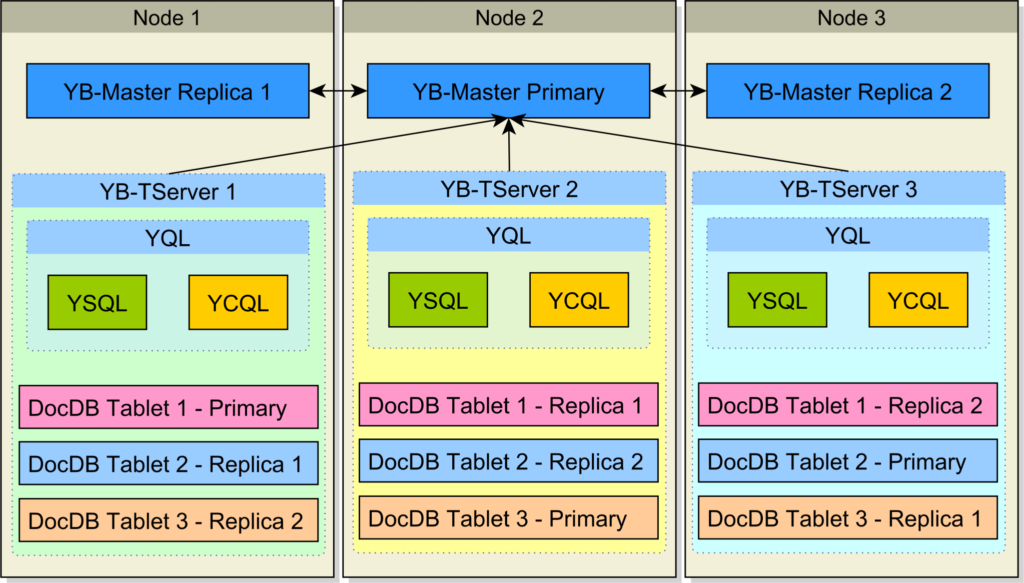
\includegraphics[width=0.8\textwidth]{resources/chapter-2/yugabyte.png}
    \caption{Arsitektur YugaByteDB \parencite{yugabyteBaeldung}}
    \label{fig:yugabyte-architecture}
\end{figure}

YugaByteDB terdiri atas Master dan TServer. Master merupakan layer kontrol yang mengatur operasi pada kluster dan metadata kluster. TServer bertugas untuk menyimpan dan mengatur data yang disimpan.
